
\documentclass[mathserif,12pt,handout,notes=show]{beamer}

\usepackage{style/beamer-en}

%
% specific settings
%

\usetheme{Singapore}
\setbeamertemplate{footline}[frame number]

% path to pictures
\graphicspath{
    {img/}
}

\begin{document}

\title{
    Some very important research
}

\author{
    \begin{tabular}{r@{ }l} 
        {Student:}           & \quad {John Doe                 } \\
        {Research Advisor:}  & \quad {Some very smart professor}
    \end{tabular}
}

\date{
    Novosibirsk, \the\year
}

\begin{frame}
    \maketitle
\end{frame}
\note{
    \lipsum[1]
}

\begin{frame}{Outline}
    \tableofcontents
\end{frame}
\note{
    \lipsum[1]
}

\section{Introduction}

\begin{frame}{Magnetotellurics}

    \begin{block}{}
        The magnetotelluric (MT) method uses surface measurements
        of natural electromagnetic fields to investigate the
        conductivity distribution of the Earth
    \end{block}
    \begin{block}{}
    \begin{columns}
        \begin{column}{0.6\textwidth}
            \begin{itemize}
                \item One of the most important tools in deep Earth research
                      (typical in the range of 500m to 10000m)
                \item Measurings have to be done for hours at each station
                      in order to get good signal to ensure high-quality data
            \end{itemize}            
        \end{column}
        \begin{column}{0.4\textwidth}
            \begin{figure}
                \centering
                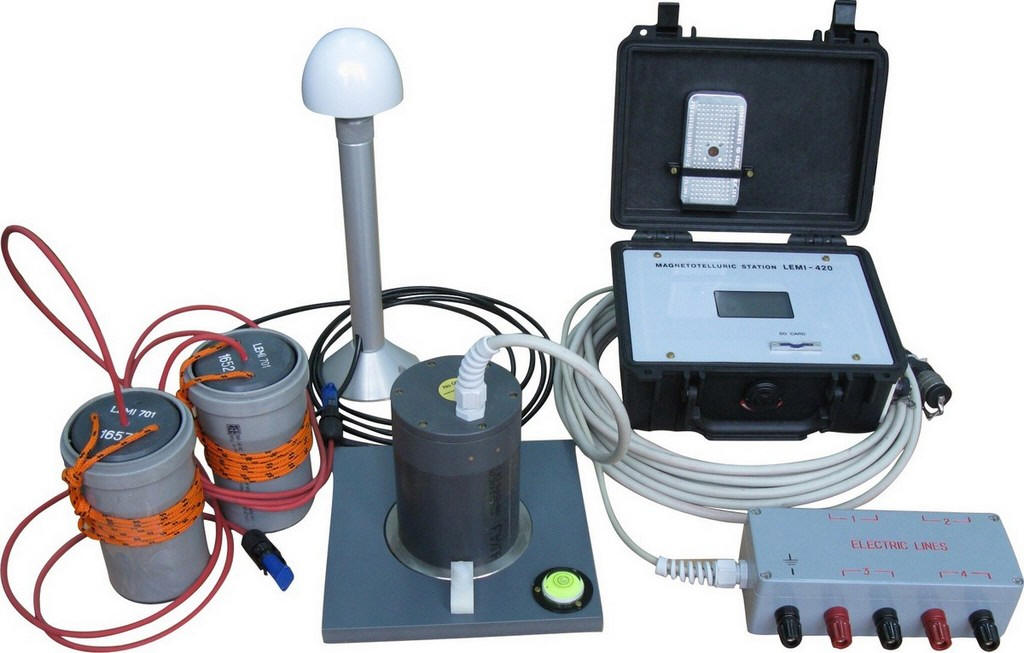
\includegraphics[width=\textwidth]{magnetotelluric-station}    
            \end{figure}
        \end{column}
    \end{columns}
    \end{block}

\end{frame}
\note{
    \lipsum[1]
}

\section{Section 1}

\begin{frame}{System of linear equations}

    \begin{columns}
        \begin{column}{0.6\textwidth}
            \begin{itemize}
                \item Most of the elements are zero
                \item Iterative methods, such as conjugate gradient method
                      and GMRES utilize fast computations of matrix-vector products
                \item One of the best methods to solve complex-valued
                      sparse systems of linear equations is COCR method
            \end{itemize}
        \end{column}
        \begin{column}{0.4\textwidth}
            \begin{figure}
                \centering
                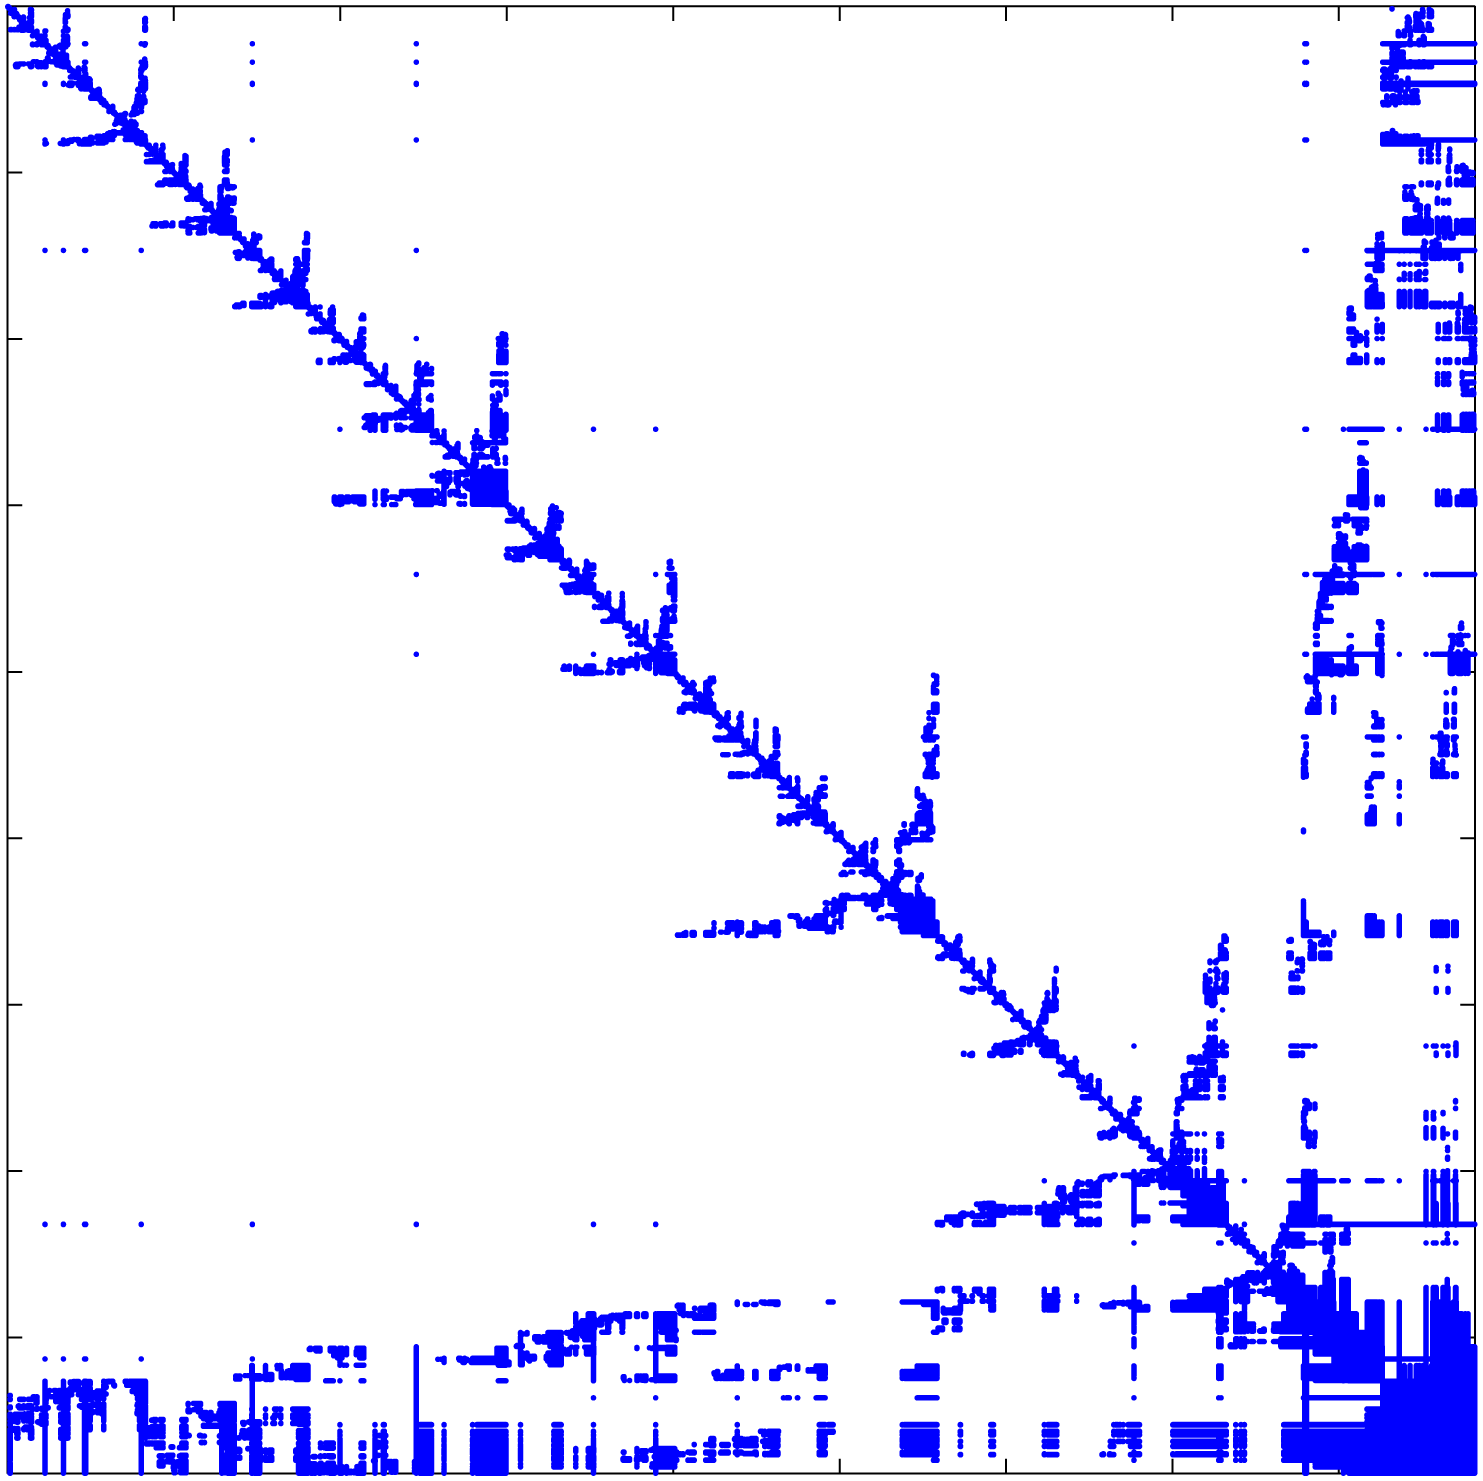
\includegraphics[width=\textwidth]{sparse-matrix}    
            \end{figure}
        \end{column}
    \end{columns}
    
\end{frame}
\note{
    \lipsum[1]
}

\begin{frame}{Acceleration methods}
 
    \begin{block}{Method 1}
        \begin{table}
            \begin{tabular}{p{0.45\textwidth} p{0.45\textwidth}}
                Method 1-1             & Method 1-2 \\
                $x=\frac{1+y}{1+2z^2}$ & $\int_0^\infty e^{-x^2} dx
                                          =\frac{\sqrt{\pi}}{2}$
            \end{tabular}
        \end{table}
    \end{block}
    \begin{block}{Method 2}
    \begin{table}
            \begin{tabular}{p{0.45\textwidth} p{0.45\textwidth}}
            $x_1 = a+b$ & $x_2=a-b $
            \end{tabular}
    \end{table}
    \end{block}
    \begin{block}{Method 3}
    \end{block}
    
\end{frame}
\note{
    \lipsum[1]
}

\section{Section 2}

\begin{frame}{Experimental}
 
    \begin{figure}
        \centering
        \begin{subfigure}[b]{0.5\textwidth}
            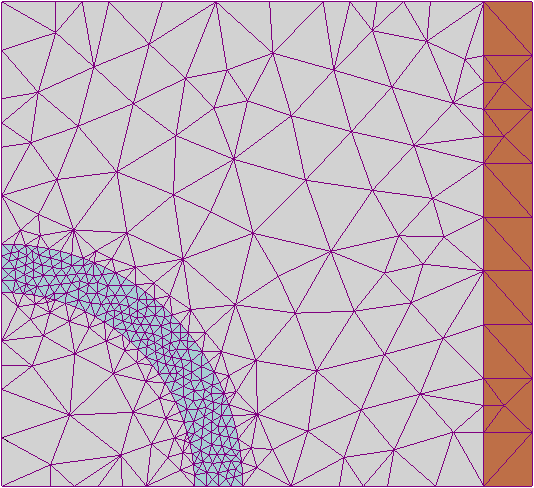
\includegraphics[width=\textwidth]{example-01}
            \caption{Computational domain}
        \end{subfigure}%
        ~
        \begin{subfigure}[b]{0.5\textwidth}
            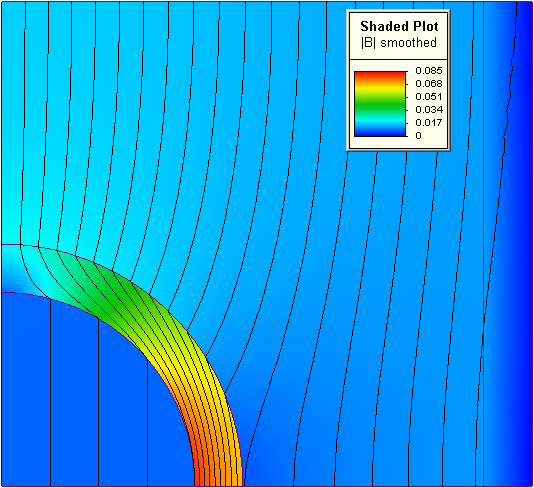
\includegraphics[width=\textwidth]{example-02}
            \caption{Finite element mesh}
        \end{subfigure}%
    \end{figure}
    
\end{frame}
\note{
	\lipsum[1]
}

\section{Conclusion}

\begin{frame}{Conclusion}
 
    \lipsum[1]
    
\end{frame}
\note{
    \lipsum[1]
}

\end{document}

